
%
% basic setup for page layout and document type
%
\documentclass[a4paper,ngerman,12pt]{scrartcl}

%
% load functionalities
% Packages
%%Paquetes
\usepackage{pdftexcmds}
\usepackage{hyperref}
\usepackage{geometry}
\usepackage{fancyhdr}
\usepackage{float}
\usepackage{tikz}
\usepackage{graphicx}
\usepackage{amsmath}
\usepackage{amssymb}
\usepackage{amsfonts}
\usepackage{multirow}
\usepackage{pgf}
\usepackage{pgffor}
\usepackage{numprint}
\usepackage[utf8]{inputenc}
\usepackage{titlesec}
\usepackage{siunitx}
\usepackage{epstopdf}
\usepackage{eso-pic}
\usepackage{amssymb}
\usepackage{pifont}





%
% geometrical setup
%
%\geometry{a4paper,lmargin=20mm,rmargin=20mm,bmargin=20mm,tmargin=20mm, includeheadfoot}


%
% define own commands
%
\newcommand{\GetAutors}{}

\newcommand{\SetLecture}[1]{%
        \newcommand{\GetLecture}{#1}%
}%

\newcommand{\SetExercise}[1]{%
        \newcommand{\GetExercise}{#1}%
}%

\newcommand{\SetLogo}[1]{%
        \newcommand{\GetLogo}{#1}%
}%

\newcommand{\AddAutor}[3]{%
        \global\edef\GetAutors{\GetAutors ,#1/#2/#3}%
}%

\newcommand*{\float}[1]{%
    \pgfmathprintnumber[%
        fixed,%
        precision=4,%
        fixed zerofill=true,%
        ]{#1}%
}%

\newcommand*{\hint}[2]{%
        \vspace{4em}{%
                \footnotesize%
                \begin{addmargin}[2em]{2em}%
                \textbf{\hspace{-2em}\footnotesize\textbf{#1}}%
                 #2%
                \end{addmargin}%
        }}

%\newcommand*{\ImageFromCache}[2]{%
%        \begin{figure}[H]%
%                \centering%
%                \includegraphics[width=15cm, height=10cm,keepaspectratio]{./cache/graphics/#1}
%                \caption{#2}%
%        \end{figure}}

\newcommand\Logo[1]{%
        \put(0,0){%
                \parbox[b][\paperheight]{10cm}{%
                        \vfill
                        %\centering
                        \hspace*{3cm}
                        \vspace*{14cm}
                        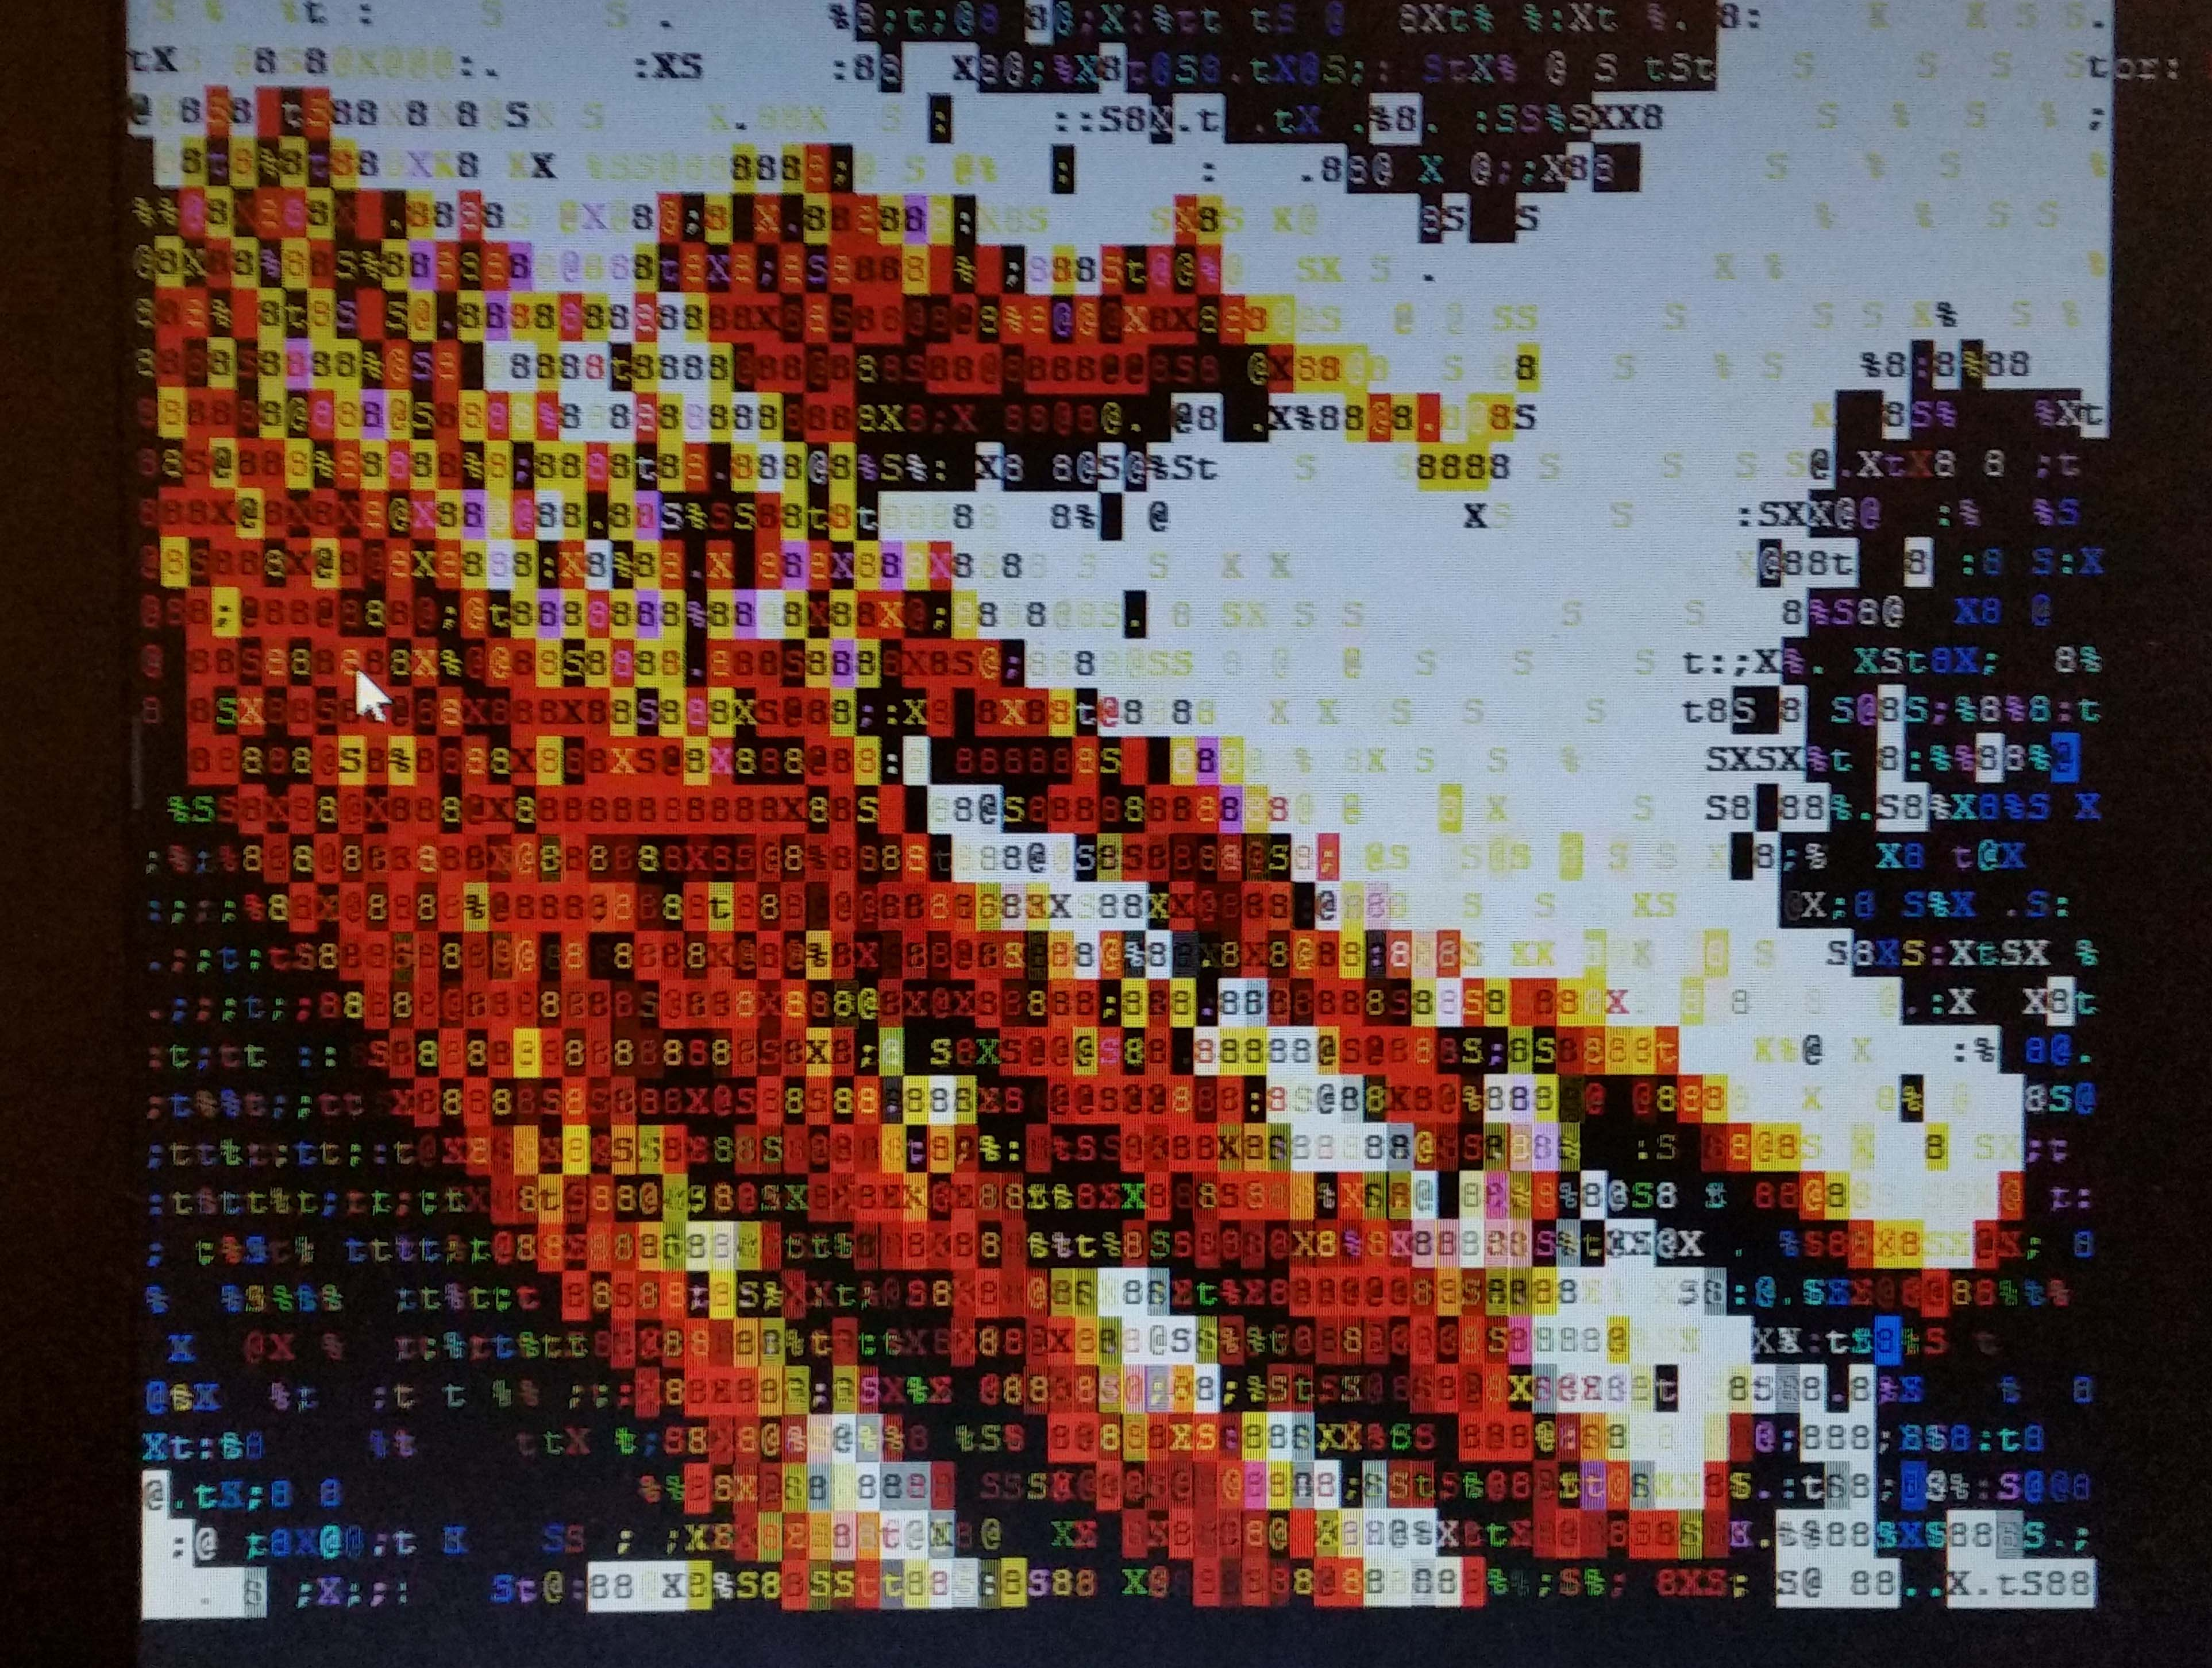
\includegraphics[width=5cm,%
                        keepaspectratio]{../UB1/images/8-8.jpg}%
                        \vfill}}}

\AtBeginDocument{%
        %
        % fancy setup
        %
        \fancyhf{}%
        \pagestyle{fancy}%
        \fancyheadoffset{1cm}%
        \fancyhead[L]{\small{\GetLecture}}%
        \fancyhead[R]{\small{Exercise \GetExercise}}%
        \fancyfoot[C]{\small{%
                \foreach \FirstName/\SecondName/\Email in \GetAutors%
                        { \FirstName \hspace{2mm}\SecondName \hspace{10mm}}}}
        \fancyfoot[R]{\small{\thepage}}%
        %
        \titleformat{\title}{\large\bfseries}{\thesection}{1em}{}%
        \titleformat{\section}{\large\bfseries}{\thesection}{1em}{}%
        \titleformat{\subsection}{\normalfont\fontsize{20}{15}\bfseries}{\thesubsection}{2em}{}%
        \titleformat{\subsubsection}{\normalfont\fontsize{18}{15}\bfseries}{\thesubsubsection}{2em}{}%
        %
        \AddToShipoutPicture*{\Logo{\GetLogo}}%
        \begin{titlepage}
        \flushright
        \rule{\linewidth}{0.5mm}\\ [0.5cm]
        {\bfseries \LARGE \GetLecture }\\
        {\bfseries \large Wintersemester 2015/2016 }\\ [2.0cm]
        {\bfseries \normalsize UNIVERSITÄT TÜBINGEN }\\ [3.0cm]

        \foreach \FirstName/\SecondName/\Email in \GetAutors
                {%
                \FirstName \hspace{2mm}%
                \SecondName%
                \hfill%
                \href{mailto:\Email}{\Email}%
                \\}
        \rule{\linewidth}{0.5mm}\\ [0.5cm]
        \flushleft
        {\bfseries \Huge Exercise \GetExercise }
\end{titlepage}
%
        \setcounter{section}{\GetExercise}
}

\newcommand{\xmark}{\ding{55}}


\SetLecture{Graphische Datenverarbeitung}
\SetExercise{1}
\AddAutor{Angel}{Rangel}{angel-eduardo.rangel-mendez@student.uni-tuebingen.de}
\AddAutor{Ido}{}{@student.uni-tuebingen.de}
\SetLogo{mb}
\graphicspath{ {images/} }

%%Inicio documento
\begin{document} 
    \begin{enumerate}
         \item[Exercise 1:] Working with images
    \end{enumerate}
    \begin{enumerate}
        \item[(a)] Write a function my loadImage that loads an image and display it (my showImage). Convert the image from uint8 to oating point representation (command double). Values should be in between 0 and 1. Use the functions image or imagesc.
    \end{enumerate}
        \\
        \\ my loadImage:
        \\  img \ = \ double(imread(filename))/255;
        \\\\ $img \ is \ a \ 3-dimensional \ MxNx3 \ matrix, \ the \ elements \ in \ img(:,:,1) \ are \ interpreted \ as \ red \ intensities, \ in \ img(:,:,2) \ as \ green \ intensities, \ and \ in \ img(:,:,3) \ as \ blue \ intensities.$
        \\\\ my showImage:
        \\ $ imagesc(img) $
        \\\\
    	\centering
        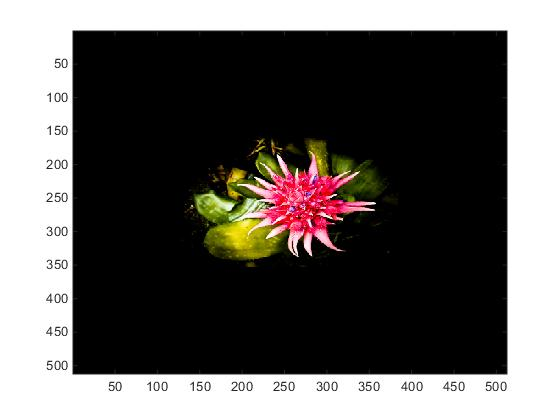
\includegraphics[scale=0.58]{images/SolutionFirstPart.jpg} 
        \\\\
    \begin{enumerate}        
        \item[(b)] Write two functions my RGBSplit and my plotRGBSplit that split the R, G and B channels of an image and display them separately. The plots should all be included in a single figure (use subplot). Each channel should be plotted in its primary color.
    \end{enumerate}
        \\\\
        \\ my RGBSplit:
        \\ split the RGB channels:
        \\ imgR = imgRGB(:,:,1);
        \\ imgG = imgRGB(:,:,2);
        \\ imgB = imgRGB(:,:,3);
        \\
        \\ my_plotRGBSplit:
        \\ [height0 , width0] = size(imgR);
        \\ [height1 , width1] = size(imgG);
        \\ [height2 , width2] = size(imgB);
        \\
        \\ Roff = struct('img', imgR, 'x', height0, 'y', width0);
        \\ Goff = struct('img', imgG, 'x', height1, 'y', width1);
        \\ Boff = struct('img', imgB, 'x', height2, 'y', width2);
        \\
        \\ Icol = imgRGB;
        \\ --figure layout
        \\ ax(1) = subplot(2,2,1);
        \\ im(1) = imshow(Roff.img);
        \\ title({'Red Channel', '[x: 0, y: 0]'});
        \\
        \\ ax(2) = subplot(2,2,2);
        \\ im(2) = imshow(Goff.img);
        \\ title({'Green Channel', '[x: 0, y: 0]'});
        \\
        \\ ax(3) = subplot(2,2,3);
        \\ im(3) = imshow(Boff.img);
        \\ title({'Blue Channel', '[x: 0, y: 0]'});
        \\
        \\ ax(4) = subplot(2,2,4);
        \\ im(4) = imshow(Icol);
        \\ title({'Original', '[x: 0, y: 0]'});
        \\\\\
        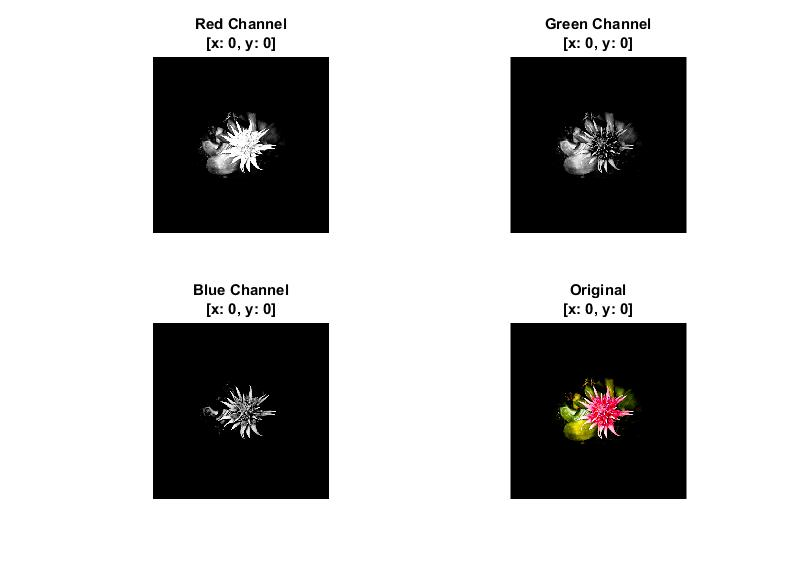
\includegraphics[scale=0.58]{images/SolutionSecPart.jpg} 
        \\
        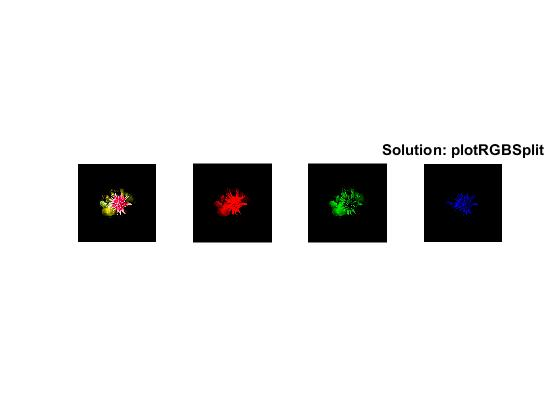
\includegraphics[scale=0.6]{images/SolutionThreethPart.jpg} 
        \\\\
    \begin{enumerate}        
        \item[(c)] Implement a gamma correction for images (my gammaCorrection).
        \\
    \end{enumerate}
        \\
        Gamma Correction:
        $$ GW = 2.2;$$
        $$ imgGC = 255*((img/255).^(1/GW))$$
     
\end{document}